\documentclass[11pt,pdftex,a4paper]{scrartcl}

\usepackage[utf8]{inputenc}
\usepackage{lmodern} 
\usepackage[T1]{fontenc}
\usepackage{microtype}

\usepackage[pdftex]{graphicx}
\usepackage{float}
\usepackage[hypcap]{caption}
\usepackage{subcaption}

\usepackage[pdftex]{hyperref} 
\usepackage{bookmark}

\usepackage{mathtools}
\usepackage{amssymb}
\usepackage{amsthm}
\usepackage{amsmath}

\usepackage{polski}
\usepackage[polish]{babel}
\selectlanguage{polish}

\hypersetup{
  colorlinks=true,
  urlcolor=blue,
}

\title{Stochastyczne Algorytmy Obliczeniowe}
\subtitle{ 
  Zastosowanie algorytmu genetycznego do rozwiązania problem replikacji danych
  w środowisku rozproszonym
}
\date{}
\author{
  Andrzej Kaczmarczyk
  \and
  Marcin Łoś
}

\begin{document}

\maketitle

\section{Wstęp}
Celem projektu było wybranie jednego problemu obliczeniowego, zapoznanie się z istniejącymi jego
rozwiązaniami, oraz próba ulepszenia któregoś z nich. Nasz wybór padł na problem replikacji danych
w systemach rozproszonych, oraz rozwiązanie oparte na algorytmie genetycznym, opisane w \cite{Ahmad}.
Na jego podstawie zaimplementowaliśmy algorytm wielopopulacyjny, oparty na modelu wyspowym. Dla danych
generowanych w sposób identyczny jak w oryginalnym artykule nie zaobserwowaliśmy znaczących zmian w 
jakości rozwiązań.

\section{Opis problemu}
Dany jest system rozproszony, składający się z \(M\) hostów \(\{H_i\}\), o pojemnościach \(s_i\), 
połączonych siecią komunikacyjną tak, że koszt przesyłu jednostki danych pomiędzy \(H_i\) i \(H_j\)
wynosi \(C(i,j)\). Istnieje także \(N\) obiektów \(\{O_i\}\), o rozmiarach \(o_i\). Host \(H_i\)
wykonuje na obiekcie \(O_k\) odpowiednio \(r^{(i)}_k\) operacji odczytu, i \(w^{(i)}_k\) operacji
zapisu. Każdy obiekt \(O_i\) znajduje się pierwotnie na jednym hoście, \(SP_i\).

Obiekty mogą zostać zreplikowane na inne hosty, tak, że suma rozmiarów obiektów zreplikowanych
na hoście \(H_i\) nie przekracza jego pojemności \(s_i\). Wszystkie hosty mają pełną wiedzę o 
replikach obiektów. Operacja odczytu obiektu \(O_k\) z hosta \(H_i\) przebiega w ten sposób, że
obiekt jest wysyłany do hosta \(H_i\) z najbliższego mu hosta zawierającego replikę \(O_k\).
Operacja zapisu natomiast odbywa się w ten sposób, że host \(H_i\) wysyła nowy stan obiektu do
hosta \(SP_k\) (pierwotnego miejsca zwierającego \(O_k\)), a ten rozsyła informację o zmianie do
pozostałych hostów zawierających repliki \(O_k\). 

Koszt sumaryczny przy danym rozłożeniu replik to suma kosztów przesyłania obiektów spowodowanego
operacjami odczytu i zapisu, przebiegającymi w opisany powyżej sposób. Koszt pojedynczego przesyłu
to iloczyn ilości przesyłanych danych (rozmiaru obiektu) i kosztu jednostkowego przesyłu między
hostami (danego przez \(C(i,j)\)). Problem polega na znalezieniu replikacji minimalizującej koszt
sumaryczny.

Nieco bardziej szczegółowy opis, wraz z wzorami na całkowity koszt znaleźć można w \cite{Ahmad}.

\section{Istniejące rozwiązania}
Problem wydaje się być problemem naturalnym i praktycznym. Pomimo tego nie istnieje wiele prac, które podejmowałyby jego temat. Być może jest to związane z jego trudnością. Dowód pokazujący trudność problemu znajduje się w \cite{newAhmad}. Szczegółowy opis algorytmu genetycznego rozwiązującego wersję statyczną problemu, znajduje się w \cite{Ahmad} oraz, rozwinięty, w \cite{newAhmad}.

Analizy oraz rozwiązania mniej ogólnych problemów tego typu dostarczają m. in. Wolfson w \cite{Wolfson}, który opisuje optymalny algorytm replikacji jednego pliku w topologiach drzewiastych czy Mahmoud, który w \cite{Mahmoud} prezentuje iteracyjne podejście w rozwiązaniu uszczegółowienia problemu DRP, FAP.

W celu uzyskania szerokiej listy rozwiązań problemów blisko powiązanych z DRP, zainteresowanych czytelników odsyłamy do przypisów w \cite{newAhmad}, w których zawartych jest kilkanaście pozycji opisujących próby rozwiązania wielu blisko spokrewnionych z DRP problemów (jednak nie samego DRP).

\section{Rozwiązanie bazowe}
Jako punkt wyjściowy przyjęliśmy rozwiązanie zaproponowane w \cite{Ahmad}. Po szczegółowy jego opis
odsyłamy do samej pracy, ta sekcja zawiera krótkie objaśnienie jego działania i używanych pojęć.

Algorytm składa się z dwóch głównych części -- algorytmu zachłannego (\textit{Simple Replication 
Algorithm}), używanego do tworzenia populacji początkowej, oraz algorytmu genetycznego (GRA).

Działanie SRA opiera się o ,,korzyść z replikacji'' (\textit{replication benefit}), stanowiącego
dla każdej party \((\textrm{obiekt}, \textrm{host})\) miarę ,,lokalnego zysku'' z replikacji tego
obiektu na tym hoście (stosunek zysku -- jak zmieni się koszt indukowany przez operacje 
\textbf{tego hosta} na tym obiekcie -- do wielkości obiektu, tj. zysk na jednostkę wielkości).
Kolejno dla wszystkich hostów wybierany jest obiekt o największym takim relatywnym zysku, i dodawana
jest do hosta jego replika, dopóki nie skończy się miejsce na hostach, bądź możliwości replikacji
z dodatnim zyskiem. Elementem losowym jest kolejność rozważania hostów, dzięki temu algorytm
nie jest całkiem deterministyczny, i może zostać użyty do wygenerowania populacji początkowej.

Algorytm genetyczny tworzy początkową populację przy pomocy SRA, a następnie symuluje jej ewolucję.
Zawiera zarówno mutację, jak i krzyżowanie. Przez \emph{gen} rozumiemy dalej ciąg bitów dla 
pojedynczego hosta, po jednym bicie na każdy obiekt, gdzie wartość bitu odpowiada istnieniu repliki
danego obiektu na tym hoście. Mutacja realizowana jest przez iterowanie po wszystkich obiektach 
i hostach, i z pewnym niewielkim prawdopodobieństwem (2\%) dodawaniu lub usuwaniu replik z hosta, 
tak by zmienić stan istniejący (odwracanie bitów w genie). Jeśli w wyniku takiego odwrócenia bitu
powstaje genom niepoprawny (schemat replikacji nie spełniający założeń), bit jest odwracany ponownie. 
Krzyżowanie to wymiana fragmentów genów pomiędzy dwoma genomami, wybranych poprzez wylosowanie w 
każdym genie dwóch punktów. Jeśli po wymianie stan jest niepoprawny, wymieniana jest reszta genu,
to wystarczy by zagwarantować poprawność rezultatu krzyżowania. Selekcja odbywa się metodą ruletkową,
z podejściem elitystycznym (kopiowanie najlepszych osobników).

\section{Modyfikacje}
Na podstawie opisanego wyżej algorytmu stworzyliśmy rozproszoną wersję wielopopulacyjną, opartą na 
modelu wyspowym -- równolegle symulowana jest ewolucja \(N\) populacji, co \(k\) kroków wymienianych 
jest cyklicznie \(m\) najlepszych osobników. W testach przyjęto odpowiednio \(N=12\), \(k=5\),
\(m=3\).

\section{Rezultaty}
W celu porównania rozwiązań osiąganych algorytmem opisanym w artykule, oraz wersji wielopopulacyjnej,
odtworzony został sposób generowania problemów testowych użyty w \cite{Ahmad}. Algorytm ten posiada
jeden parametr \(U\), opisujący procent operacji będących zapisem (testy przeprowadzane były dla 
\(U\in\{0.02, 0.05, 0.1\}\)). Koszty połączeń między hostami 
losowane są z rozkładem jednostajnym ze zbioru \(\{1,\ldots,10\}\). Dla każdego obiektu losowany
jest host stanowiący jego pierwotną lokację. Dla każdej party obiekt-host losowana jest ilość odczytów
(rozkład jednostajny na \(\{1,\ldots,40\}\)). Na podstawie sumarycznej ilości odczytów \(R\) losowana
jest ilość zapisów -- liczba z przedziału \(\{\frac{1}{2}W,\ldots,\frac{3}{2}W\}\), gdzie 
\(W = R\,U\). Zapisy te są następnie losowo rozdzielane pomiędzy pary obiekt-host. Wielkości obiektów
są losowane z rozkładem jednostajnym ze zbioru \(\{15,\ldots,55\}\). Niech \(S\) będzie łącznym 
rozmiarem wszystkich obiektów. Pojemności hostów losowane sa z 
\(\{\frac{1}{2}CS,\ldots,\frac{3}{2}CS\}\), gdzie \(C=0.15\).

Poniższe wykresy przedstawiają wyniki osiągnięte przy użyciu podstawowej wersji algorytmu.
Widać na nich kolejno: ilość stworzonych replik (średnia ilość replik na obiekt), oraz zysk (jaki 
ułamek kosztu całkowitego pozwoliło zaoszczędzić stworzenie replik) przy stałej ilości obiektów (150),
i zmiennej ilości hostów. Są analogiczne do tych umieszczonych w artykule bazowym, brak jednak wykresu
obrazującego zysk przy stałej ilości hostów i zmiennej ilości obiektów, ze względu na bardzo duży czas
obliczeń (wada języka Python). Algorytm genetyczny skonfigurowany był na stworzenie 10 pokoleń.

\begin{figure}[H]
    \centering
    \begin{subfigure}[b]{0.49\textwidth} 
        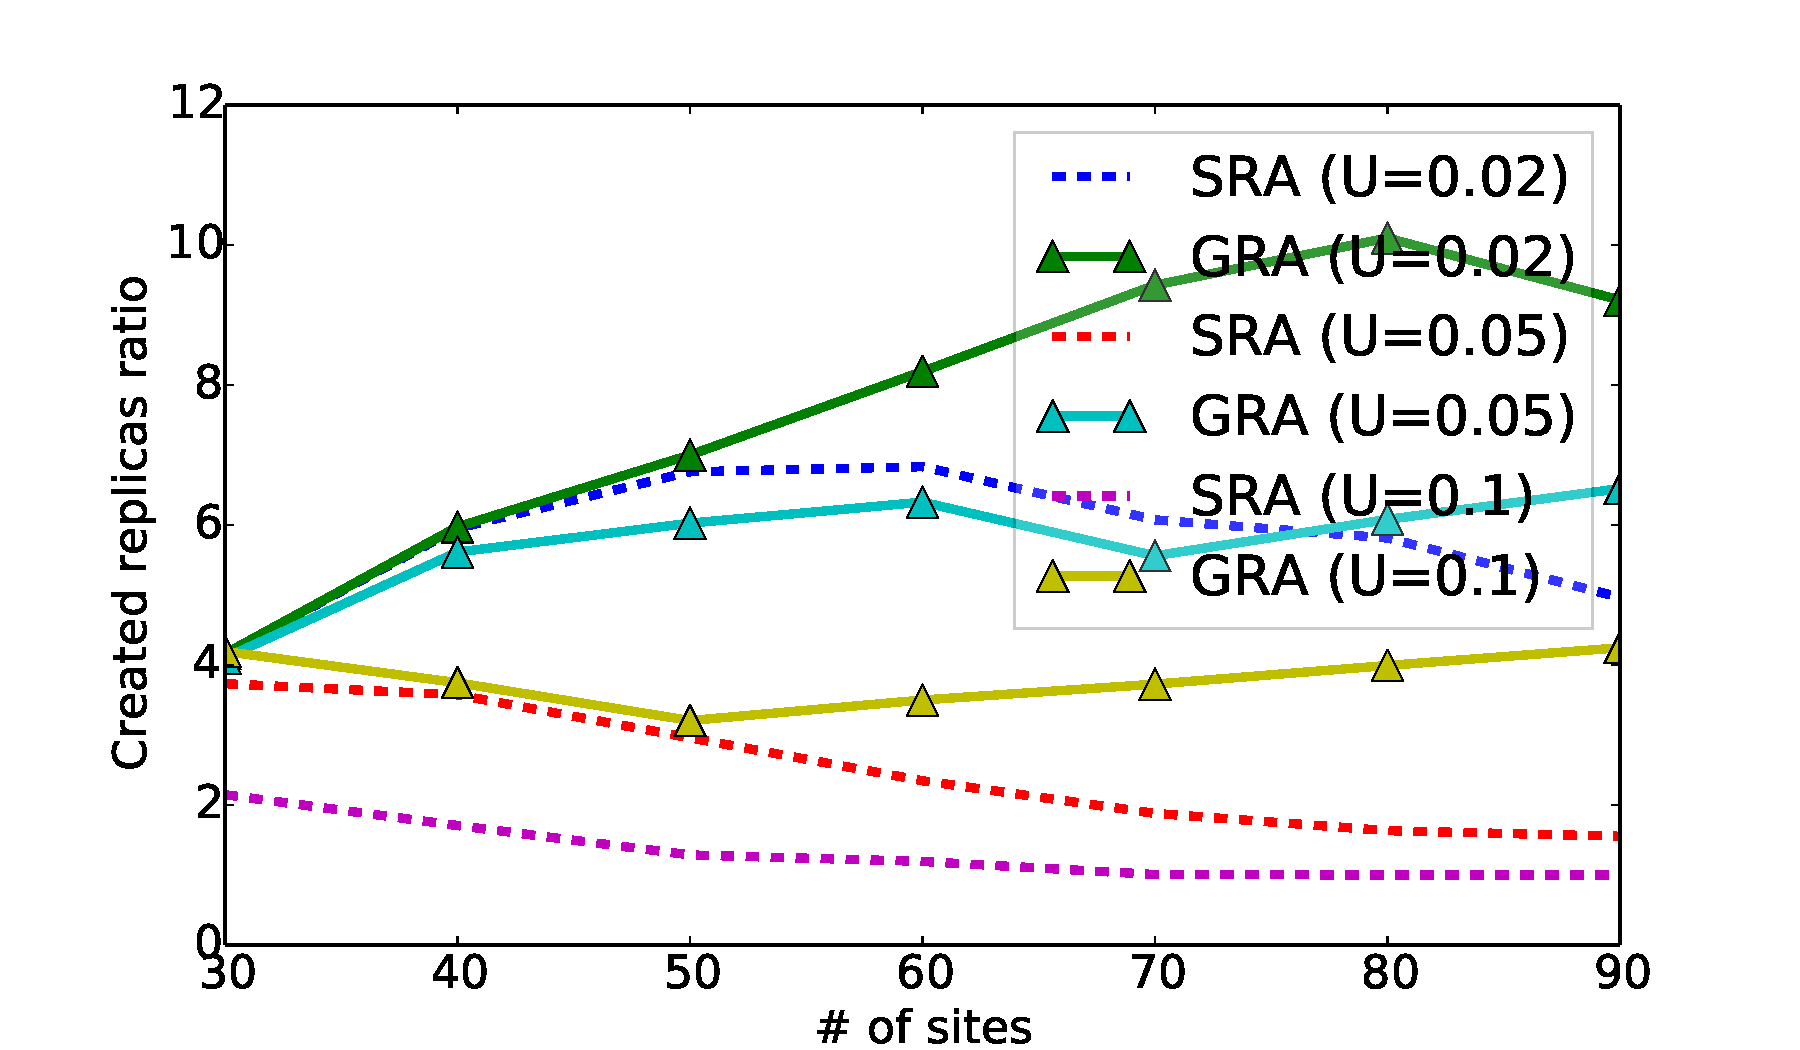
\includegraphics[width=\textwidth]{plots/replicas}
        \caption{ilość stworzonych replik}
    \end{subfigure}
    \begin{subfigure}[b]{0.49\textwidth}
        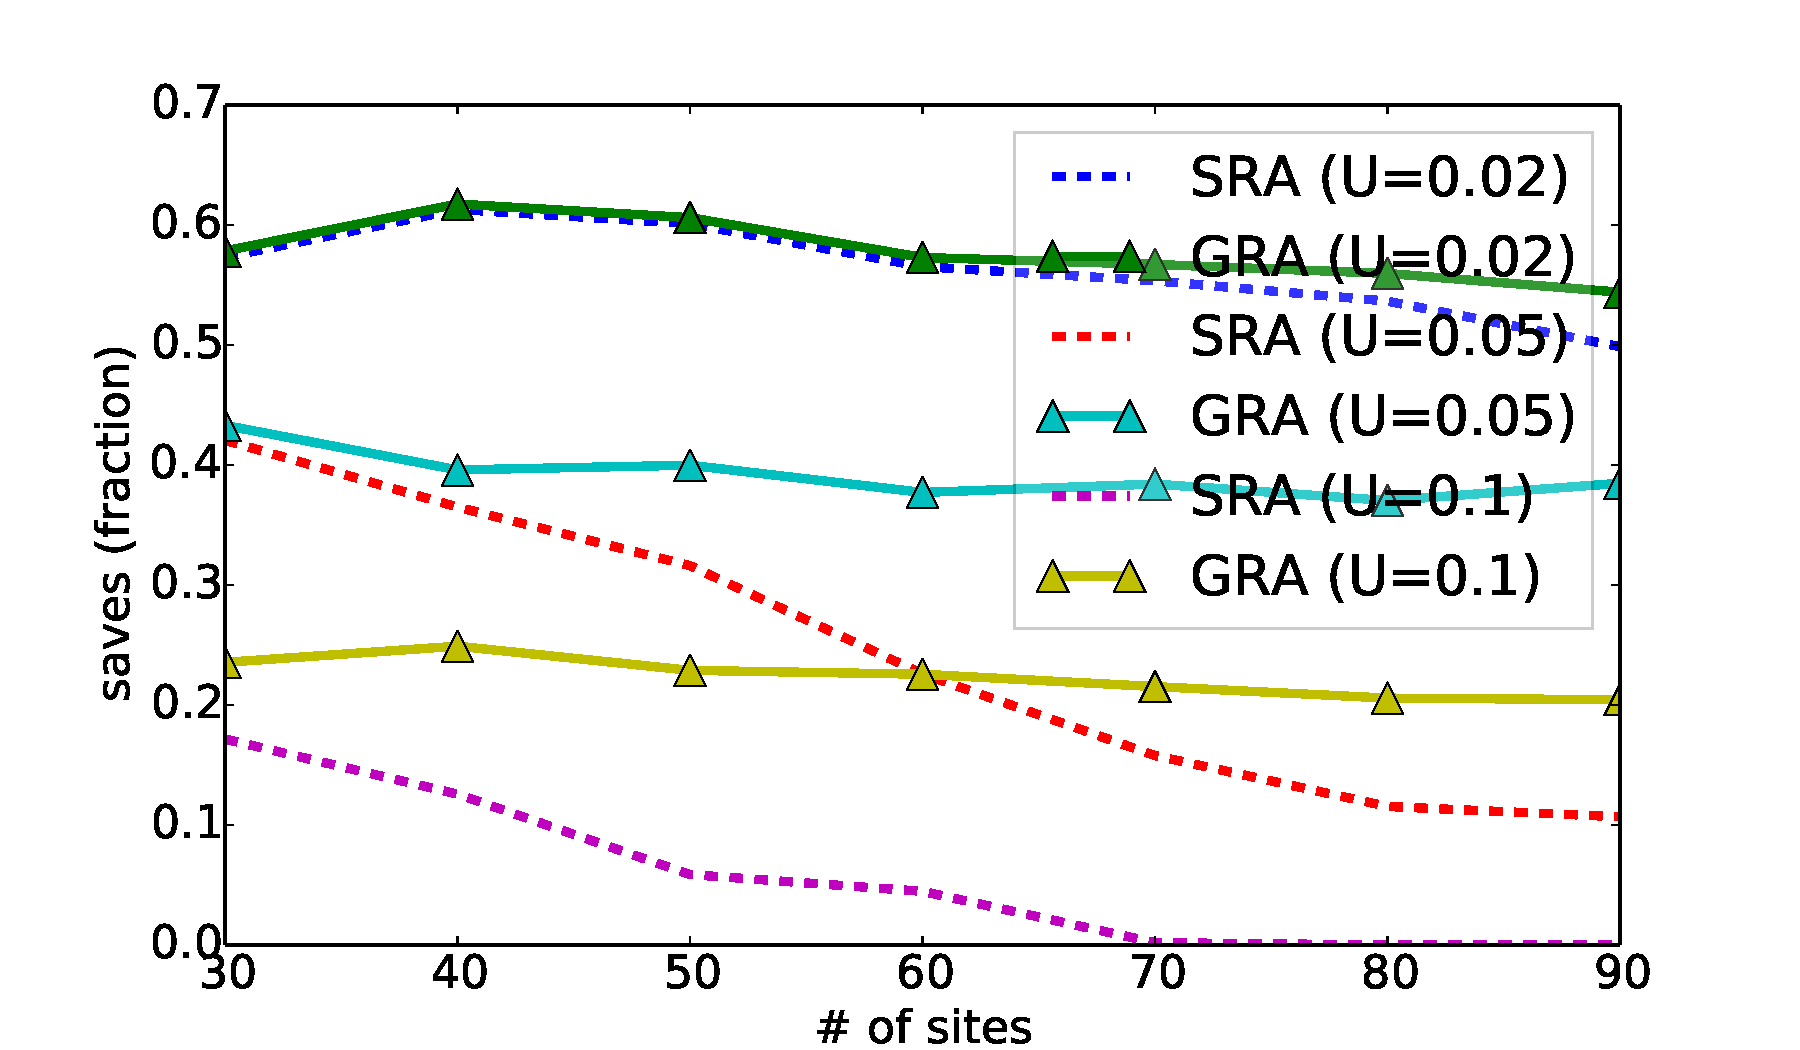
\includegraphics[width=\textwidth]{plots/saves}
        \caption{zysk z replik}
    \end{subfigure}

    \caption{Wyniki dla algorytmu z artykułu}
    \label{plot:original}
\end{figure}


Testy wersji wielopopulacyjnej przeprowadzone zostały na komputerze Zeus, z użyciem 12 rdzeni (12 
populacji, po jednej na instancję programu), zasymulowane zostało 20 pokoleń.

\begin{figure}[H]
    \centering
    \begin{subfigure}[b]{0.49\textwidth} 
        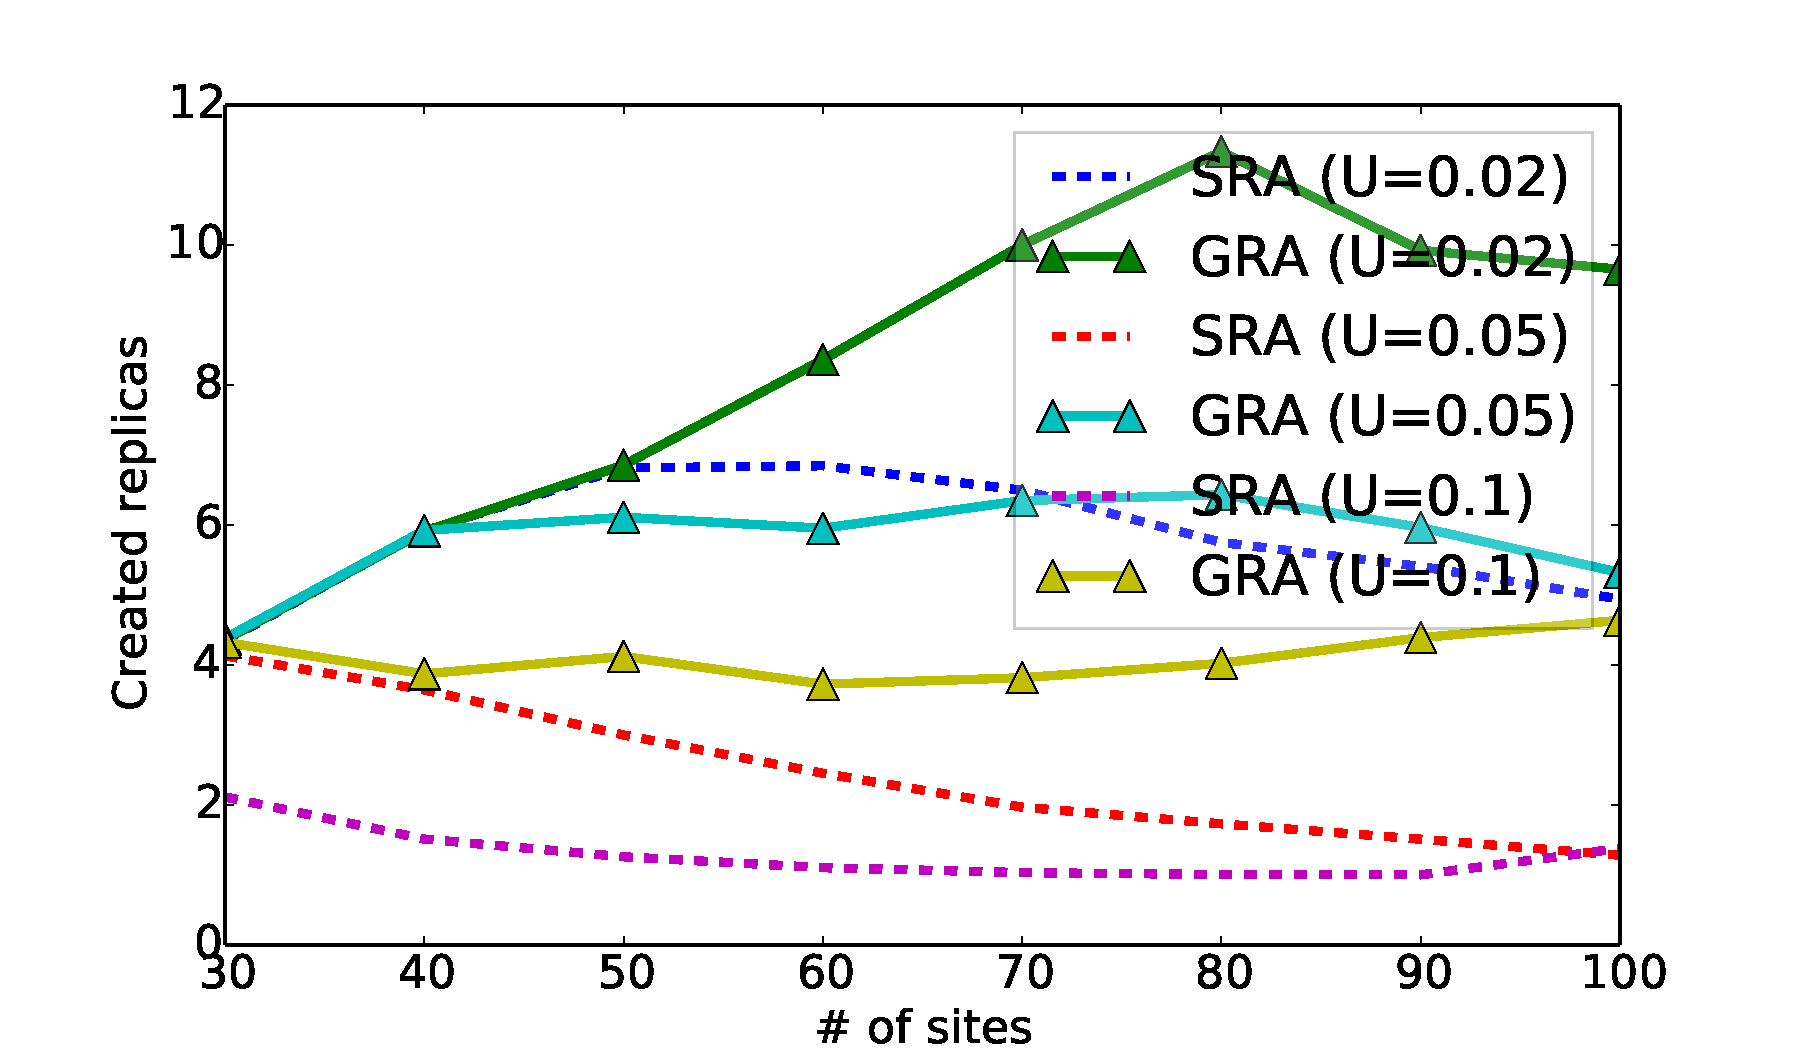
\includegraphics[width=\textwidth]{plots/replicas_isl}
        \caption{ilość stworzonych replik}
    \end{subfigure}
    \begin{subfigure}[b]{0.49\textwidth}
        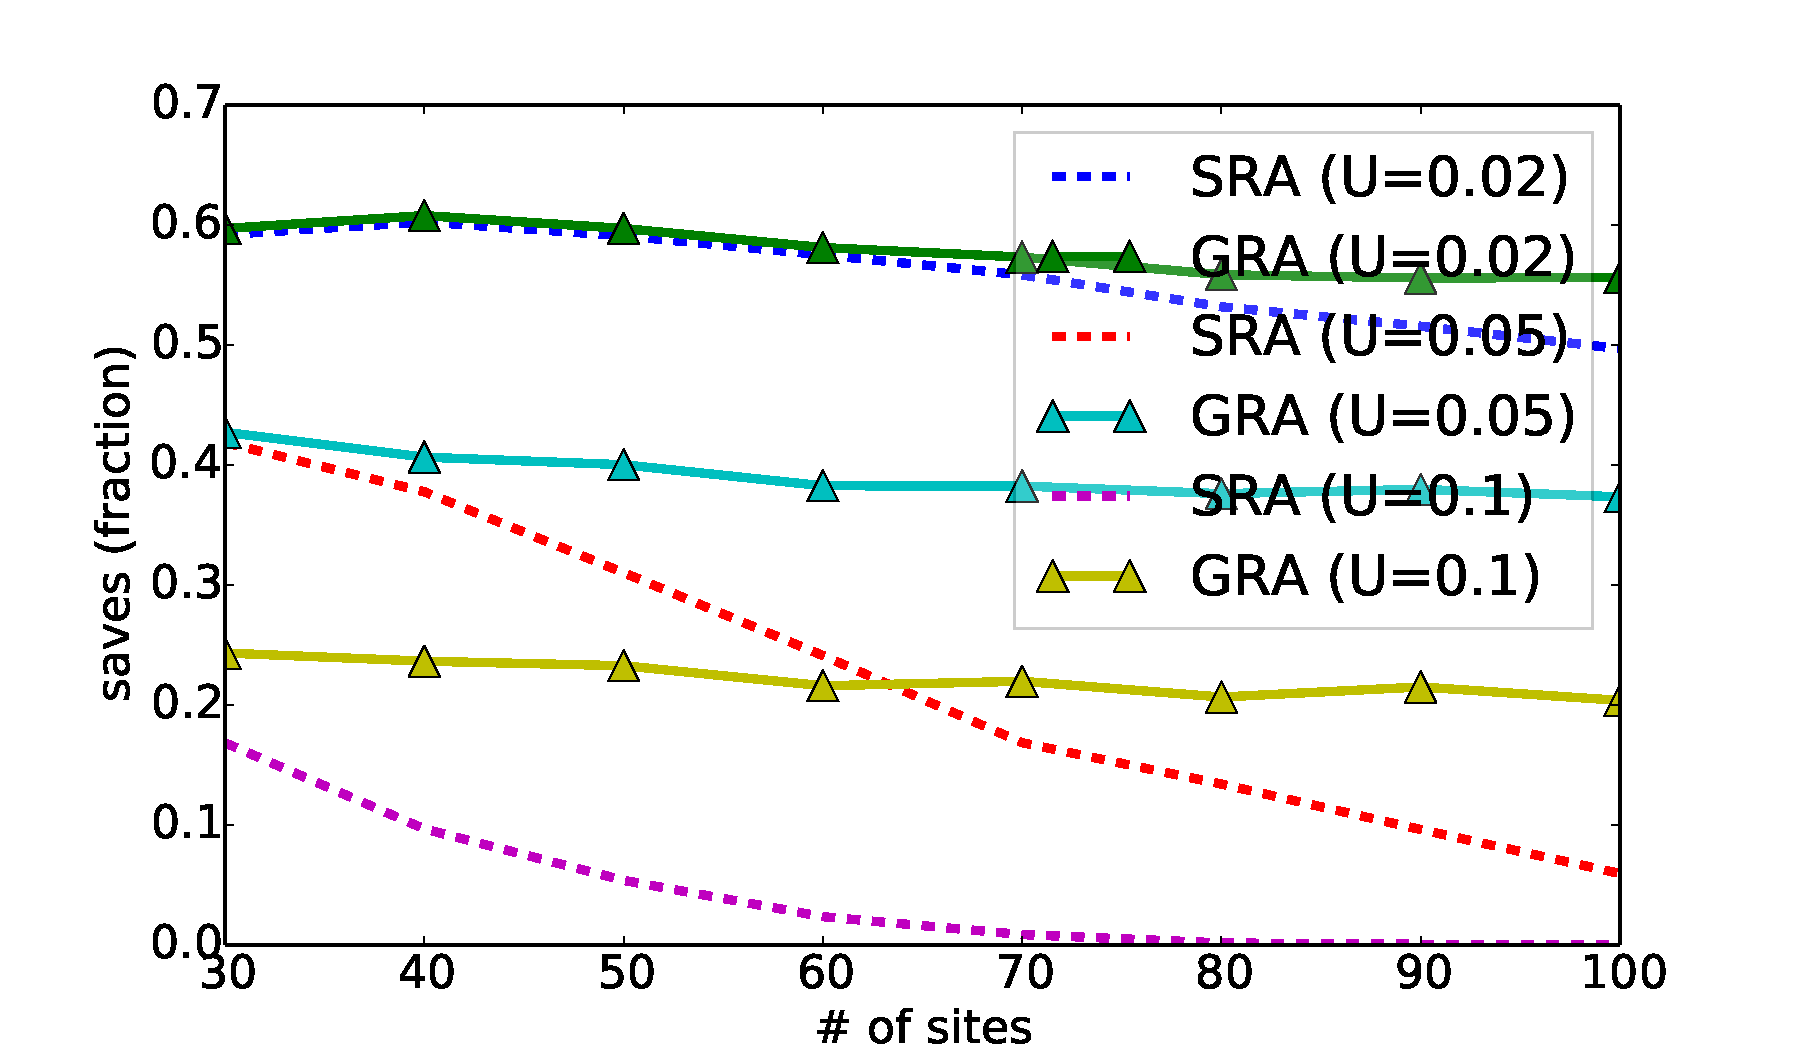
\includegraphics[width=\textwidth]{plots/saves_isl}
        \caption{skalowane}
    \end{subfigure}

    \caption{Wyniki dla algorytmu wyspowego}
    \label{plot:original}
\end{figure}

\begin{figure}[H]
    \centering
    \begin{subfigure}[b]{0.49\textwidth} 
        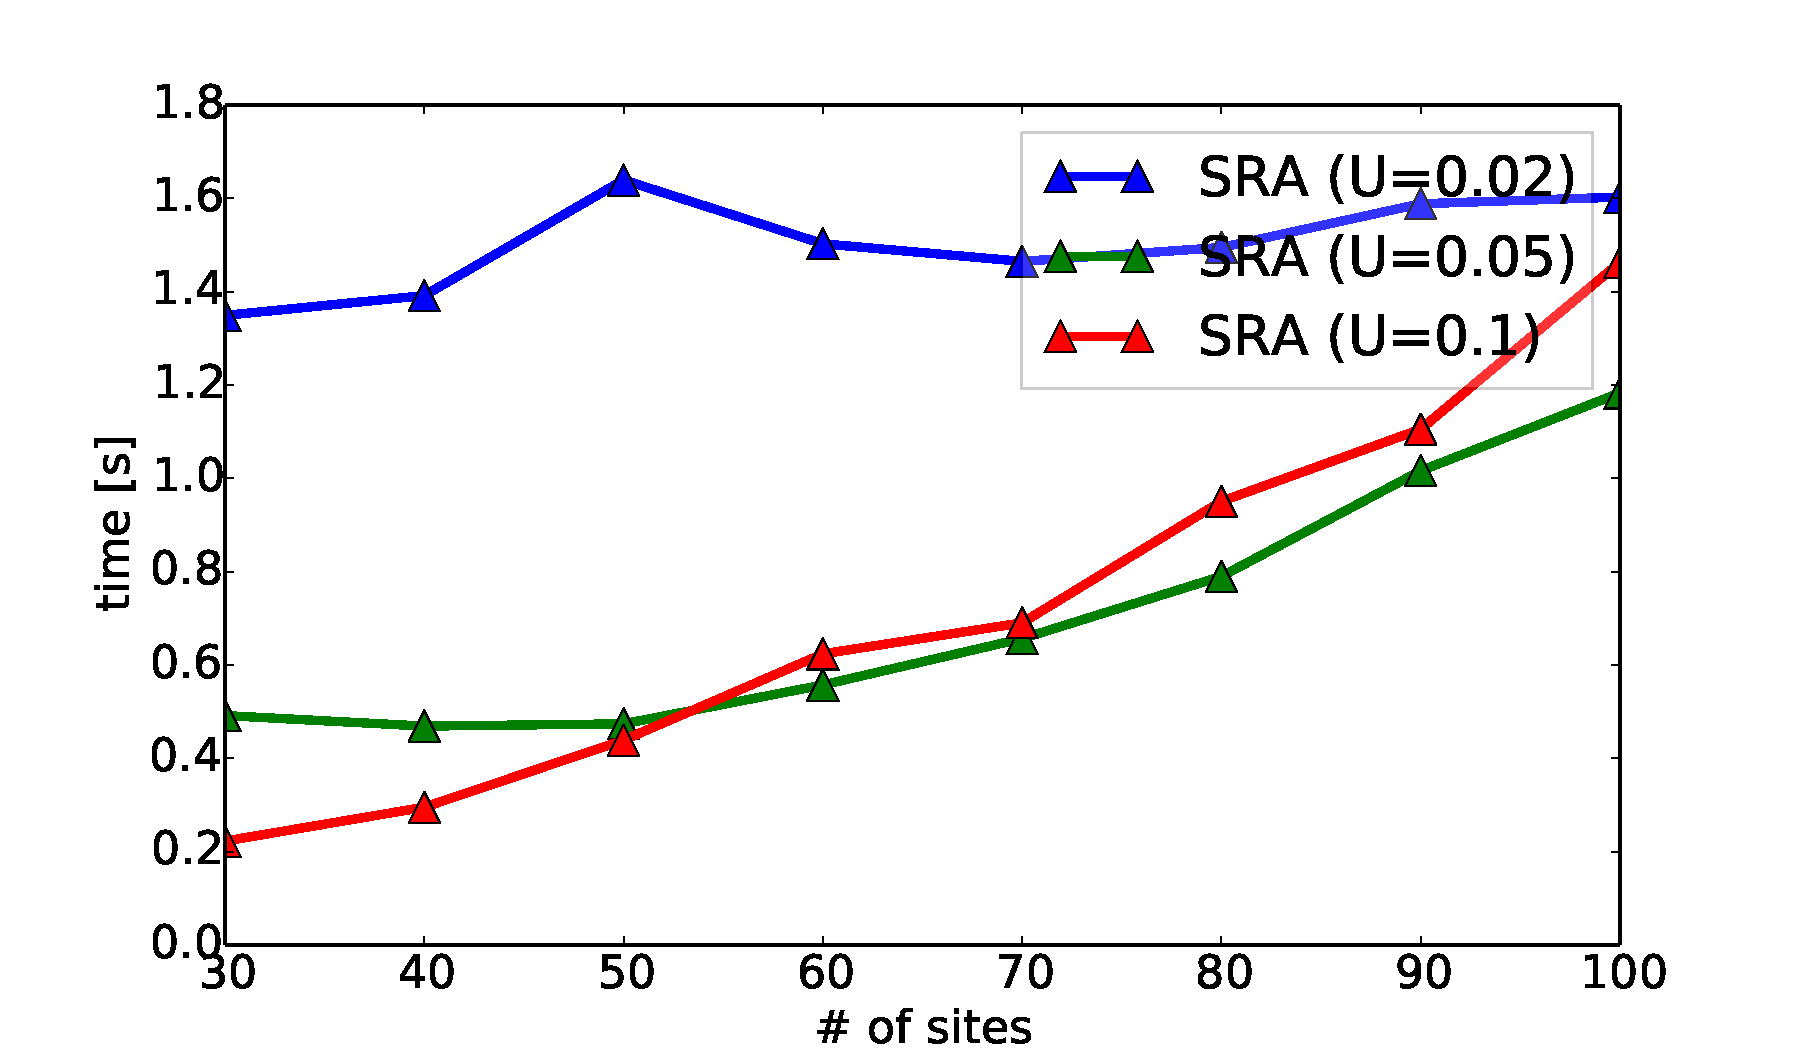
\includegraphics[width=\textwidth]{plots/time_sra_isl}
        \caption{ilość stworzonych replik}
    \end{subfigure}
    \begin{subfigure}[b]{0.49\textwidth}
        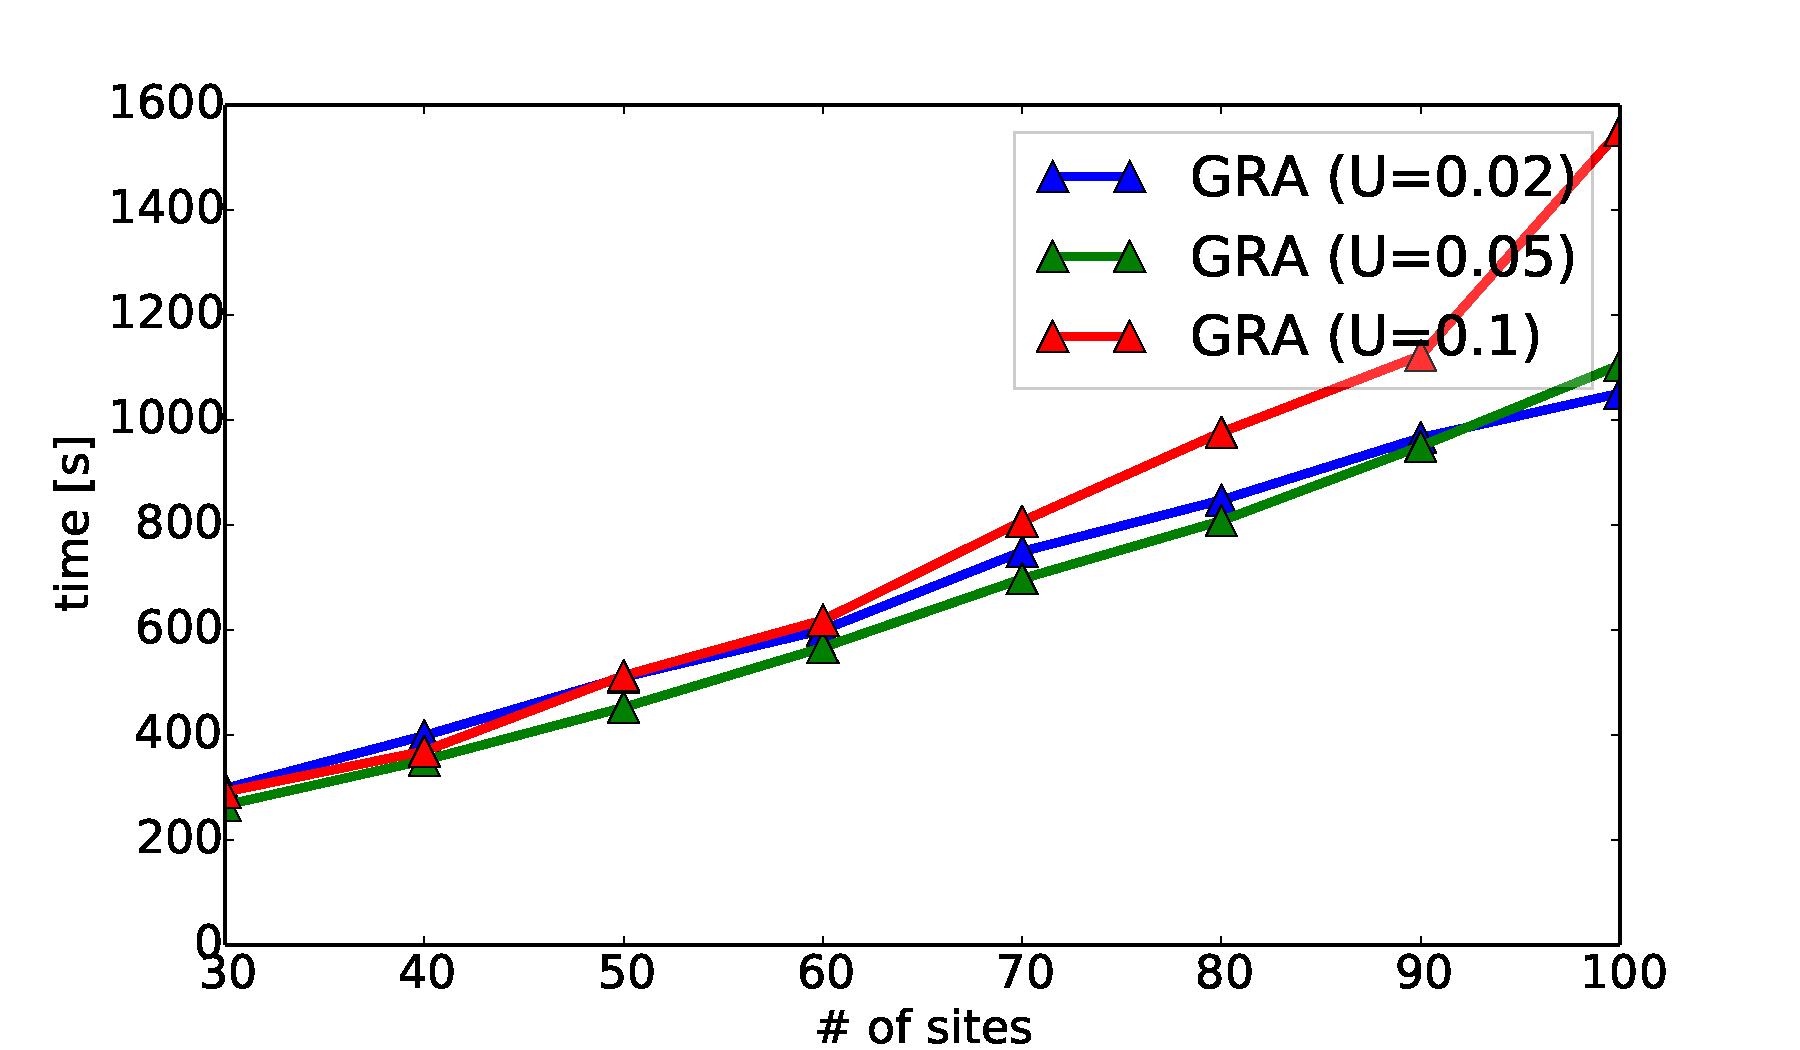
\includegraphics[width=\textwidth]{plots/time_gra_isl}
        \caption{skalowane}
    \end{subfigure}

    \caption{Czasy działania algorytmu wyspowego}
    \label{plot:original}
\end{figure}

Jak widać na powyższych wykresach, zastosowanie algorytmu wielopopulacyjnego nie przyniosło zauważalnej
poprawy w otrzymanych rozwiązaniach.


\section{Uwagi}
Początkowo planowaliśmy użyć nieco innego generatora danych do testów, takiego, który w naszym odczuciu
mógłby lepiej odwzorowywać własności instancji problemu, które występować mogą w praktyce. Dobranie 
jednak parametrów tak, by zaobserwować wyniki podobne do tych przedstawionych w artykule bazowym okazało
się trudne, w związku z czym odtworzyliśmy wiernie sposób generacji danych w nim opisany. Po tym zabiegu
udało nam się odtworzyć dość dobrze oryginalne wyniki. 

Podczas prac nad programem rozważaliśmy także możliwość redukcji problemu do problemu ILP oraz zastosowanie jednego z szeroko dostępnych solverów liniowych. Zdecydowaliśmy się na tą próbę, ponieważ problem (szczególnie dokładne wzory na obliczenie sumarycznego kosztu) mocno przypominał, na pierwszy rzut oka, równanie liniowe. Po nieudanych próbach okazało się jednak, że nie byliśmy w stanie przedstawić problemu w formie, która odpowiada problemom typu ILP, więc pomysł porzuciliśmy.

\section{Narzędzia}
Do realizacji implementacyjnych aspektów projektu wykorzystaliśmy język Python i bibliotekę
PyEvolve \cite{pyevolve}, dostarczającą różnych komponentów (np. strategie selekcji) pozwalających
budować algorytmy genetyczne. Do implementacji rozproszonej użyte zostało MPI, za pośrednictwem
Pythonowych bindingów udostępnianych przez bibliotekę mpi4py \cite{mpi4py}.

\section{Podsumowanie}

Zastosowanie algorytmu wielopulacyjnego opartego na modelu wyspowym nie przyniosło żadnych widocznych
korzyści. Istnieje kilka możliwych przyczyn takiego stanu rzeczy. Po pierwsze, trudno powiedzieć, na
ile znajdowane rozwiązania dalekie są od rozwiązania optymalnego -- przy niewielkiej ilości operacji
zapisu algorytm obniża koszt sumaryczny o ponad połowę, niewykluczone, że rozwiązanie optymalne nie
jest znacząco od niego lepsze. Przemawia za tym także fakt, że wyniki z 10 pokoleń wersji podstawowej
i 20 pokoleń wersji wyspowej nie różnią się mimo dwukrotnego wydłużenia czasu ewolucji każdej z
populacji.

Inną możliwą przyczyną jest niewielkie zróżnicowanie populacji na poszczególnych wyspach. Populacje
wybierane są niezależnie przy użyciu tego samego schematu, i są raczej na tyle duże (80 osobników),
że trudno się spodziewać, by istotnie się od siebie różniły. Stąd, jedyną w zasadzie korzyścią z modelu
wyspowego jest zrównoleglenie obliczeń -- w pewnym sensie uruchamiamy (prawie) ten sam algorytm
na wielu maszynach, dzięki czemu mamy szansę znaleźć lepsze rozwiązanie. Nie sposób jednak oczekiwać
jakichś spektakularnych różnic.


\section{Możliwe kierunki rozwoju}

W trakcie realizacji projektu nie wszystkie pomysły zrodzone w czasie dyskusji i przemyśleń zostały
zrealizowane. Najistotniejsze kwestie są omówione w kolejnych akapitach.

Jakkolwiek algorytm wyspowy nie przyniósł żadnej obserwowalnej poprawy jakości otrzymywanych rozwiązań,
w pewnym stopniu może być to spowodowane małym zróżnicowaniem populacji na poszczególnych wyspach.
Niewykluczone, że stworzenie populacji bardziej zróżnicowanych (poprzez modyfikację rozkładów, z których
są losowane --tj. przez użycie różnych sposobów ich inicjalizowania) przyniosłoby lepszy efekt.

Jednym z pomysłów, które ostatecznie nie zostały wprowadzone w życie, była relaksacja operacji
genetycznych (mutacji i krzyżowania), polegająca na tym, by wymuszanie poprawności rozwiązań niejako
przenieść do etapu ewaluacji -- dopuszczać wszystkie stworzone osobniki, jednak stosować kary przy
ewaluacji, tak, by osobnikami o największym fitnessie były osobniki z poprawnym genotypem, jednak by
zwiększyć ,,mobilność'' populacji -- umożliwić zmiany genotypu, które bez relaksacji nie byłyby 
możliwe, i tym samym być może pozwolić na odkrycie trudnych do znalezienia minimów.

Otwarta pozostaje kwestia znalezienia lepszych operatorów mutacji i krzyżowania, bardziej dostosowanych
do rozpatrywanej przestrzeni stanów. Był to jeden z pierwszych pomysłów, jednak nie osiągnęliśmy w tym
kierunku żadnych postępów. Znalezienie sensownych operatorów wewnętrznych (nie wychodzących poza --
dość nieregularną -- przestrzeń stanów) pozwoliłoby uprościć algorytm, a ze względu na pewną 
,,kompatybilność'' z przestrzenią stanów być może także polepszyć znajdowane przez ich użycie 
rozwiązania. Wydaje się to być jednak zadanie stosunkowo trudne, i trudno na chwilę obecną powiedzieć,
jakiego rodzaju operacji można by szukać.

Przemyśleć należałoby kwestię generowania danych testowych. Nasze początkowe próby przeprowadzane
były na danych generowanych inaczej, niż w artykule, jednak wróciliśmy do niego by odtworzyć wyniki
i przy nim pozostaliśmy. Nie jest on jednak w naszym odczuciu idealny. W szczególności obiekcje 
budzić może topologię połączeń -- w artykule bazowym odległości \(C(i,j)\) pomiędzy poszczególnymi
hostami są losowane z rozkładem jednostajnym ze zbioru \(\{1,\ldots,10\}\). Najbardziej oczywistym
problemem zdaje się być pogwałcenie nierówności trójkąta -- \(C\) nie jest metryką. Trudno powiedzieć,
w jaki sposób wpływa to na używany algorytm, jednak wydaje się prawdopodobnym, że mogą istnieć jakieś
zmiany/ulepszenia, dla których jest to istotne. 

\begin{thebibliography}{}

  \bibitem{Ahmad} 
  T. Loukopoulos I. Ahmad.
  \emph{Static and Adaptive Data Replication Algorithms for Fast Information Access in 
    Large Distributed Systems}

  \bibitem{pyevolve}
  Biblioteka PyEvolve,
  \url{http://pyevolve.sourceforge.net/0_6rc1/}

  \bibitem{mpi4py}
  Biblioteka mpi4py,
  \url{http://mpi4py.scipy.org/}
  
  \bibitem{newAhmad} 
  T. Loukopoulos I. Ahmad.
  \emph{Static and adaptive distributed data replication using genetic algorithms}

  \bibitem{Wolfson} 
  O. Wolfson, S. Jajodia, Y. Huang.
  \emph{An adaptive data replication
algorithm}

  \bibitem{Mahmoud}
  S. Mahmoud J.S. Riordon.
  \emph{Optimal allocation of resources in
distributed information networks}



\end{thebibliography}

\end{document}